\documentclass[preprint1]{aastex}
% \documentclass{princeton_astro_thesis}
\usepackage[printonlyused]{acronym}
\usepackage{amsthm}
\usepackage{amsmath}
\usepackage{amsfonts}
\usepackage{verbatim}
\usepackage{mathtools}
\usepackage{float}
\usepackage{graphicx}
\usepackage{xcolor}
\usepackage{url}
\usepackage{solarized-light}
\usepackage[caption=false]{subfig}
\usepackage{rotating}

\newcommand\pcp{\mbox{ pc}^{-3}}
\newcommand\Msun{\; M_\odot}
\newcommand\msun{\; M_\odot}
\newcommand\Myr{\mbox{ Myr}}
\newcommand\Gyr{\mbox{ Gyr}}
\newcommand\pc{\mbox{ pc}}
\newcommand\gram{\mbox{ g}}
\newcommand\nbody{\texttt{NBody6++GPU }}


\numberwithin{equation}{section}
\setkeys{Gin}{width=\linewidth,totalheight=\textheight,keepaspectratio}
\graphicspath{{graphics/}}

\title{}
\author{Elias Rubin}
\begin{document}
% running out of time because black hole mass is the seed mass 
% at redshift above 7 we already see MBh around a billion solar masses
% need half Gyr tops.  So M seed must be ~10^4-10^5
% Lbh, quasar is some constant times black hole mass
% hence there is an observational constraint

\section{Scientific Motivation} \label{Intro}


Observations of high redshift ($z \ge 6$) quasars hosted by supermassive black holes (SMBHs) 
of masses in excess of a billion solar masses 
present a major theoretical challenge.
To illustrate, as an example, 
a seed BH of mass $10^4\msun$ would need a duty cycle of 100\%
accreting at 113\% Eddington rate 
from redshfit $z=15$ in order to reach 
the observed mass of $2\times 10^9\msun$ 
of quasar ULAS J1120+0641 at $z=7.1$ \citep[][]{2011Mortlock}.
Similarly demanding accretion arrangements are required for some other
cases, including 
the observed quasar SDSS J0100+2802 of SMBH mass of $1.2\times 10^{10}\msun$ at $z=6.3$ \citep[][]{2015Wu}
and 
quasar ULAS J1342+0928 of SMBH mass of $0.8\times 10^{9}\msun$ at $z=7.1$ \citep[][]{2017Banados}.

Clearly, black holes of masses $\sim 10-100\msun$ formed by normal massive stars,
when they end their lives,
provide inadequate seeds for these observed SMBHs at the epoch of reionization \citep{2003Bromm, 2013Hosokawa}. 
To explain SMBHs with masses over $10^9 \Msun$ forming under $1 \Gyr$, 
BH seeds of masses around $>10^4\Msun$ formed at redshift $z\ge 10$ are needed.

In this work we examine the scenario of formation of very massive stars
($10^5-10^8\msun$) 
through the process of runaway collisions in 
a subset of dense and massive globular clusters (GCs) formed at very high redshift.
Sufficiently dense clusters are highly collisional, and provide for the possibility of runaway growth. 
As a single star continues to increase in mass and stellar radius, it increases the likelihood of further collisions, and provides an avenue for runaway star growth \citep{2015Katz}. 
This mechanism for very massive black hole formation is one of two that are commonly considered, 
the other being the direct collapse of gaseous clouds, as described in \citet{2003Bromm}.
Although direct collapse black holes have been investigated as a promising path to SMBH formation, 
\citet{2016Latif} and others raise questions about the viability of that pathway because of significant radiation feedback effects which can reduce the rate of mass accretion below the $0.1 \Msun/\mbox{yr}$ required to develop sufficiently large seed mass black holes.

We perform calculations of stellar dynamics and stellar collisions in globular clusters with direct N-Body simulations 
and extend the scenario of runaway stellar collisions to 
the formation of very massive mass stars, beyond the intermediate mass ($\sim 10^3\msun$) BHs 
as previously demonstrated by \citet{2004SPZ}.

An important requirement for a possible runaway formation of very massive stars
is to have significantly larger collision cross sections of stars.
This requirement then translates to 
a stringent time constraint.
For a normal stellar initial mass function (IMF)
it can be shown that the collision cross sections are dominated by the most massive stars.
It is thus our expectation, which is verified by our simulations later,
that in order to achieve a runaway collision sufficient dense and massive globular clusters
are required such that the runaway collisions occur in the first few million years before
massive stars end their lives and lose most of their collision cross sections.
For a typical initial mass function with a maximum mass of $\sim100 \Msun$, this time is about $3 \Myr$, 
afterwards stellar evolution effects such as supernovae and stellar winds can be expected to prevent runaway \citep{2002SPZ}. 

Very massive ($\ge 10^4\msun$) stars, once formed,
will ultimately shortly collapse, due to general relativistic instability \citep{1964Chandrasekhar},
to become SMBHs.
These SMBHs will anchor the centers of massive galaxies 
and grow primarily by accreting gas from their surroundings at rates probably fairly close to the Eddington rate
to become the observed billion solar mass SMBHs powering the quasars at $z>6$.
Occasionally, mergers of galaxies may also help somewhat grow the SMBHs.


%\citet{2002SPZ} suggests runaway collisions as a pathway to \ac{IMBH} formation, with runaway masses at approximately $0.1\%$ of the total cluster mass in the clusters simulated.  \citet{2004SPZ} 
%\textbf{Should observational constraints or other literature be discussed in this section?  What about more detail about alternative \ac{SMBH} pathways like in Latif?}
%\textbf{Cite for relationship between quasar luminosity and black hole mass?}


\section{Parameter Space of Globular Clusters}
\label{Model}

Globular clusters are some of the densest stellar systems in the universe. 
The GCs in the Milky Way come in two distinct flavors,
one which is on average more spherically distributed, has low metallicity 
and low rotation, the other which on average possesses an opposite set of properties
\citep[][]{1985Zinn}.
The former sub-population has an age of $\sim 12-13$Gyr and is thus believed
to have formed at the epoch of reionization ($z>6$).
The stellar dynamics in the context of runaway stellar collisions,
right after the formation of this old GC population, is the subject of our study.


The overall picture of a runaway collision proceeds approximately in the following way
after the formation of a GC.
Initially, the stellar distribution is unsegregated in terms of stellar mass.
Subsequently, gravitational interactions between stars, a process called dynamical friction,
cause more massive stars to lose
kinetic energy to gradually towards the center of the GC, with lighter stars moving outwards in compensation.
The ability of allowing massive stars to move to the central region is critical, because
massive stars have the largest collision cross sections and the central region is densest.
Therefore, two of the most important parameters that likely determine whether
a runaway collision occurs or not 
are the dynamical friction time at the half-mass radius, $t_{DF}$, and the density profile of the GC.

The density profiles of observed GCs are often approximated as 
a \citet[][]{1911Plummer} or \citet[][]{1962King} profile.
For our purpose we choose the King profile due to its ability to easily parameterize
the central region of a GC, where most of the collision action occurs.
In their investigation of collision in 
UCDs MGG-9 and MGG-11, \citet{2004SPZ} identify two factors about collisional clusters that can lead to supermassive star formation: 
concentration parameter $w$ and dynamical time $t_{\mathrm{df}}$.
For a GC with a King profile, we have three key parameters:
the concentration parameter $c$, total mass $M$ and $t_{DF}$, 
with $c$ and $t_{DF}$ defined as 

\begin{subequations}
    \begin{align*}
    c &\equiv \log{\frac{R_t}{R_c}} \\
    t_{\mathrm{df}} &\equiv \frac{\langle m \rangle}{M_*} \frac{0.138N}{\ln{0.11M/100\Msun}}\left(\frac{R^3}{GM}\right)^{1/2}
    \end{align*}
\end{subequations} 
\noindent
where $M_*$ is the mass of massive stars that migrate inward via dynamic friction;
we choose $M_*=100\msun$ to define $t_{df}$.


We stress that all three parameters are important. In particular,
the collision rate per time that determines the outcome 
depends not only on $c$ and $t_{DF}$ but also on $M$.

{\bf you need to add some text about the King profile and how $C$ is related to the gravitational potential well depth.}
 
We survey the parameter space of $C$, $t_{DF}$ and $M$, in part guided by observations.
But we imagine that some of the densest and most massive globular clusters may have disappeared from 
our sight to have integrated into larger stellar systems that are no longer recognized as GCs today.
Observationally, the GCs and ultra compact dwarf galaxies (UCDs), which are essentially more massive cousins
of GCs observed beyond the Local Group, span a mass range of $10^5-10^{8.5}\msun$.  
Well known GCs 47 Tuc and $\omega$~Cen have $c=2.03$ and $1.30$ \citep[][]{2000Carraro}, respectively,
falling in the overall range of $c\sim 1-3$ \citep[e.g.,][]{2007Evstigneeva}.
We thus sample the range $1-3$ for the parameter $c$.
The parameter $t_{DF}$ is a function of GC mass $M$, half-mass radius $R$ and the mass of the star in question $<m>$
(see equation above).






\section{Simulation Methods} \label{Methods}

\subsection{The N-Body Problem}
We are interested in following the evolution of collisional clusters and exploring the range of parameters in which they can lead to \ac{SMBH} formation. Finding a solution entails solving the equation of motion for each particle specified by the force $\mathbf{F}_{i}$ and its time derivative $\mathbf{F}^{(1)}_{i}$ as follows:
\begin{subequations}
    \begin{align}
    \mathbf{F}_{i} &= -m_{i}\sum_{i \neq j} Gm_{j} \frac{\mathbf{R}}{R^3}; \\
    \mathbf{F}^{(1)}_{i} &=  -m_{i}\sum_{i \neq j} Gm_{j} \left[ \frac{\mathbf{V}}{R^3} + \frac{3\mathbf{R}(\mathbf{V} \cdot \mathbf{R})}{R^5}\right],
    \end{align}
    \label{eqn:gravmotion}
\end{subequations}
where $G$ is the gravitational constant, $m_j$ is the mass of particle $j$, and $\mathbf{R}$ and $\mathbf{V}$ are the vector distance and velocity respectively between any two particles $i$ and $j$.  Because it is not possible to analytically solve the dynamical equations for every body in a cluster, systems must be evolved numerically. Developing numerical methods for N-Body simulations is a long tradition, but the two most popular methods are tree-based simulations and direct simulations. The tradeoff between the two is one of computational cost versus accuracy. Notwithstanding implementation details, direct simulations compute pairwise force terms for every pair of bodies at each discrete simulation timestep, which comes with a computational cost per timestep of $O(N^2)$ in the number of particles.  Tree-based simulations partition the simulation space and compute pairwise terms for close neighbors of a given particle, but aggregate forces from groups outside of a close radius. Thus, the cost per timestep goes as $O(N\mathrm{log}N)$.

The metric generally used for simulation error is energy conservation across the system. Practicioners focus their efforts on increasing simulation speed while keeping increases to errors within acceptable bounds. The acceptable level of error depends on the problem domain and desired fidelity of the result.  For our cluster simulations we have many bodies in close proximity and care about the accurate treatment of close encounters, binaries, multiple systems, and collisions, so we use \nbody, a direct code.  An alternative we considered is the tree-based code \texttt{Starlab}, but our initial testing and recommendations from practicioners suggested that \nbody would be better for our use case.

We perform direct N-body simulations over a range of cluster parameters varying in total mass, half-mass radius, and concentration.  We use the \texttt{McLuster} software of \citet{2011Kupper} to generate initial conditions and the \nbody software of \citet{2015Wang} to evolve the clusters. We also describe some modifications to the \nbody software made in attempts to accelerate simulations.

\subsection{Numerical Methods}
\nbody is the latest version in a family of direct N-body simulators beginning with \texttt{NBody1} of \citet{1963Aarseth}. \citet{1999Aarseth} describes in detail the evolution of the \texttt{NBody} family of programs and numerical methods therein.  The code is written primarily in Fortran but has modules written in CUDA for GPU extensions and C++ for access to AVX/SSE instructions. It is parallelized with OpenMP.

In order to solve equations~\ref{eqn:gravmotion}, the \nbody integrator uses a direct fourth-order Hermite integration method, as well as a hierarchical block step \citep[][and refs within]{2015Wang}. This is a kind of adaptive timestep system. Instead of evaluating all particles at every timestep, particles are binned into quantized groups, and only those particles at an integer multiple of their timestep are integrated. This speeds up the integration of slow moving particles, while still allowing for accuracy for more extreme particles. The code uses the neighbor scheme of \citet{1973Ahmad} to speed up the integration further by separating into the more economical regular force (forces on a body generated by bodies outside a neighbor radius) and irregular force (forces generated by bodies within a neighbor radius). In \nbody, the regular force computations are done on the GPU, and irregular force computations are done on the CPU with the AVX/SSE library of \citet{2012Nitadori}. The next part of this section explains each of these in more detail.

The Hermite integration method is used to solve equations~\ref{eqn:gravmotion}.  This is a predictor-corrector method that uses a third-order Taylor expansion.  The expression for the force is described in \citet{1999Aarseth} and is as follows:

\begin{subequations}
\begin{align}
    \mathbf{F}_{t+1} &= \mathbf{F}_{t} + \mathbf{F}^{1}_{t}\Delta t + \frac{1}{2}\mathbf{F}^{(2)}_{t}\Delta t^2 + \frac{1}{6}\mathbf{F}^{(3)}_{t}\Delta t^3, \\
    \mathbf{F}^{(1)}_{t+1} &= \mathbf{F}^{(1)}_{t} + \mathbf{F}^{(2)}_{t}\Delta t + \frac{1}{2}\mathbf{F}^{(3)}_{t} \Delta t^2.
\end{align}
\label{eqn:LowOrderHermite}
\end{subequations}
$\mathbf{F}$ and $\mathbf{F}^{(1)}$ can be computed at the beginning and end of a timestep by using equations~\ref{eqn:gravmotion}. They are used to form the higher order terms
\begin{subequations}
\begin{align}
    \mathbf{F}^{(2)}_{t} &= \frac{2}{\Delta t^2}\left[-3(\mathbf{F}_{t} -\mathbf{F}_{t+1}) - 2(\mathbf{F}^{(1)}_{t} + \mathbf{F}^{(1)}_{t+1}) \Delta t\right], \\
    \mathbf{F}^{(3)}_{t} &= \frac{6}{\Delta t^3}\left[2(\mathbf{F}_{t} - \mathbf{F}_{t+1}) + (\mathbf{F}^{(1)}_{t} + \mathbf{F}^{(1)}_{t+1})\Delta t\right].
\end{align}
\label{eqn:HigherOrderHermite}
\end{subequations}
Then the predictor and corrector $\mathbf{r}_{p, t+1}, \mathbf{v}_{p, t+1}, \Delta \mathbf{r}$, and $\Delta \mathbf{v}$ are given thusly
\begin{subequations}
\begin{align}
    \mathbf{r}_{p, t+1} &= \mathbf{r}_{t} + \mathbf{v}_{t} \Delta t + \frac{1}{2} \mathbf{F}_{t} \Delta t^2 + \frac{1}{6} \mathbf{F}^{(1)}_{t} \Delta t^3, \\
    \mathbf{v}_{p, t+1} &= \mathbf{v}_{t} + \mathbf{F} \Delta t + \frac{1}{2}\mathbf{F}^{(1)}_{t} \Delta t^2, \\
    \Delta \mathbf{r} &= \frac{1}{24} \mathbf{F}^{(2)}_{t} \Delta t^4 + \frac{1}{120}\mathbf{F}^{(3)}_{t} \Delta t^5, \\
    \Delta \mathbf{v} &= \frac{1}{6} \mathbf{F}^{(2)}_{t} \Delta t^3 + \frac{1}{24}\mathbf{F}^{(3)}_{t} \Delta t^4,
    \end{align}
\label{eqn:PredCorr}
\end{subequations}
with the final state at $t+1$ given by $\mathbf{r}_{t+1} = \mathbf{r}_{p, t+1} + \Delta \mathbf{r}$ and $ \mathbf{v}_{t+1} = \mathbf{v}_{p, t+1} + \Delta \mathbf{v}$. 

The Hermite predictor is used for each time step in the hierarchical block step scheme. Block steps are the way the \texttt{NBODY} family of codes addresses the large dynamic range in the velocities and proximities of bodies in clusters. This is necessary for performance because otherwise the time step for the entire system would be determined by the separation of the closest bodies. Instead each particle is given its own timestep using the following formula of \citet{2017Khalisi} 

\begin{equation}
\Delta t_{i} = \sqrt{\eta \frac{\lvert \mathbf{a}_{1,i}\rvert \lvert \mathbf{a}^{(2)}_{1,i}\rvert + \lvert \mathbf{a}^{(1)}_{1,i} \rvert ^2}{\lvert \mathbf{a}^{(1)}_{1,i} \rvert \lvert \mathbf{a}^{(3)}_{i,1} \rvert \lvert \mathbf{a}^{(2)}_{1,i}\rvert^2}}.
\label{eqn:blocksteptime}
\end{equation}

We use an initial value of $0.01$ for $\eta$ which we arrived at as it generally allowed our simulations to progress further before energy error becomes too great which forces a restart.  This value may be further adjusted if the relative energy error $dE$ (defined as the difference in total simulation energy between checkpoint times) becomes close (within a factor of 5) to the maximum tolerance $Q$. The correction factor is given by $\sqrt{dE/Q}$.  Our simulations use a checkpoint timestep of $0.01$ $t_{\mathrm{nb}}$, where $t_{\mathrm{nb}}$ is the simulation time unit and is equal to $\frac{1}{2\sqrt{2}} t_{\mathrm{df}}$ \citep{2017Khalisi}. We set $Q=0.05$, which allows for a maximum energy error of $20\%$, and causes a readjustment of $\eta$ when the energy error reaches $4\%$.

Figure~\ref{fig:blockstep} shows an example of how the particles are advanced. 
\begin{figure}
    \centering
    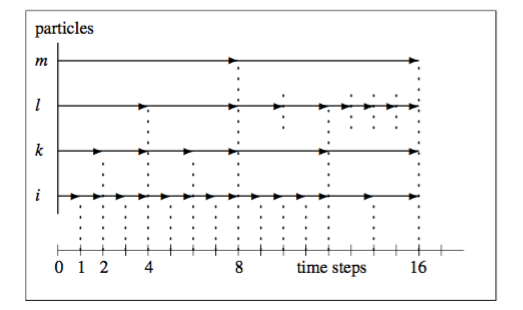
\includegraphics[width=\textwidth]{KhalisiTimeStep}
    \caption{Particles $i$, $k$, $l$, and $m$ have separate time steps. A full force computation is done at each arrow, otherwise, the position and velocity are extrapolated from the values already computed.  These time steps are reevaluated by equation~\ref{eqn:blocksteptime} after a full integration cycle. Subsystems which are evaluated independently are replaced by their center of mass in the block scheme. Figure reproduced from \citet{2017Khalisi}.}
    \label{fig:blockstep}
\end{figure}

The \nbody employs the neighbor scheme of \citet{1973Ahmad} in conjunction with the Hermite integrator and block timestep. This is a further optimization to speed up the calculations, this time by identify particles that are spatially close to each other. Thus, a given particle will actually have two timesteps, a regular timestep and (smaller) irregular timestep. Particles have a neighbor list of size at most $N_{\mathrm{nb}} \ll N_{\mathrm{tot}}$.  These are advanced using a similar predictor-corrector as the Hermite scheme above, computing the full force for neighbor particles and the last regular values for non-neighbors. Membership in the neighbor list is determined by the size of the neighbor sphere and the length of the neighbor list $N_{\mathrm{nb}}$.  The first $N_{\mathrm{nb}}$ particles within a sphere of radius $r_{\mathrm{search}}$ are included.  We found that too small values for $N_{\mathrm{nb}}$ would lead to code crashes and settled on a value of 1024.  We use a search sphere of radius $1 \times 10^{-4} \pc$.

The distinguishing feature of the \texttt{NBODY} family is their use of \citet{1965Kusta} (KS) regularization to generate solutions for binaries, triples, and multiple systems with high levels of accuracy.  This treatment for close encounters adds a good deal of complexity to the implementation, but the scheme essentially works by searching for bodies closer to each other than $r_{\mathrm{min}}$, replacing them in the next integration step by their center of mass, and integrating them separately at a smaller timescale and in a different reference frame. This is useful to avoid numerical truncation errors caused by bodies being too close in the originally reference frame. The KS regularization is extended to multiple systems and adds perturbing bodies using a variant of the \citet{1973Ahmad} neighbor scheme. KS pairs and multiples are terminated if the distance between the bodies exceeds $r_{\mathrm{min}}$ or if the bodies collide, in which case they are merged.  We discuss the merger criteria and method later in this section.

Although \nbody uses MPI parallelization to scale across multiple compute nodes, there are some sequential bottlenecks including KS regularization. In our experiments, we experienced no gain from using multiple nodes, and it's possible that the KS regularization method was responsible. We touch on this further in section~\ref{conclusions}.

We performed our simulations on the \texttt{Tiger2} GPU cluster at Princeton University. Most experiments were performed on one compute node which each use four NVIDIA Tesla P100 GPUs and 2.4 GHz Broadwell processors parallelized with OpenMP.

\subsection{Initial and Boundary Conditions}
We generate our initial conditions using the \texttt{McLuster} software of \citet{2011Kupper}. For the initial distribution of positions and velocities, we use a \citet{1966King} profile, varying half-mass radius and concentration.  We use the initial mass function of \citet{2001Kroupa} which degenerates to a Saltpeter IMF above $0.5 \Msun$.  For our simulations with cluster mass $2 \times 10^5 \Msun$, we use a mass range of $1$ to $100 \Msun$.  For cluster mass $6 \times 10^5 \Msun$, we increase the lower bound to $3.3 \Msun$.  For cluster mass $2 \times 10^6 \Msun$, we use a lower bound of $13 \Msun$ and an upper bound of $120 \Msun$.  We do not apply an external tidal field, initialize primordial binaries, or apply primordial mass segregation. 

We use an open boundary condition so particles that do escape do not return to the simulation. Our escape condition is a distance from center of greater than twice the tidal radius. Both of these conditions remain uniform over all of our simulations.

\subsection{Merger Scheme}
The default merger criteria in \nbody follows that of \citet{1992Kochanek}.  For a two-body system with pericenter $R_p$, the bodies are merged if

\begin{equation}
 \frac{R_{p}}{R_{1}} \leq 1.3 \times (\frac{M_T}{2M_1})^{1/3}.
 \label{eqn:kochanekcriteria}
\end{equation}

This merger scheme is conservative.  In the case of a central mass with $m = 200 \Msun$ (a typical case after a couple of mergers) and an additional mass with $m = 1 \Msun$, and using $r_{\mathrm{central}} = (\frac{m}{\Msun})^{0.55}$, we would not merge the two stars unless they had a pericenter distance smaller than $20$ stellar radii, or a deviation of only about $3\%$ from the radius of the central mass.

In an effort to increase the speed of our simulations by spending less time in KS regularization for insignificant bodies, we experimented with short-circuiting this merger scheme for pairs meeting certain conditions.  We experimented with merging binaries where one member was $5$ or $10$ times larger than the other, provided the pericenter distance was smaller than $10 r_\mathrm{large}$ (in the more conservative trial) and $100 r_\mathrm{large}$ in the more liberal one.  We avoided merging with the central mass, but did want to reduce the number of KS pairs for peripheral bodies. We found that the overall runtime was not affected significantly by this change to the merger scheme. Simulation results appeared robust to the factor $10$ difference, but were affected by the factor $100$ difference.  We tested changes to our merger scheme at approximately the transition between collisional and non-collisional clusters: a mass of $2 \times 10^5 \Msun$, a concentration of $2$, and a half-mass radius of $2.9 \pc$.

\subsection{Verification}
\citet{2009Anders, 2012Anders} perform comparisons between \texttt{NBody4} of \citet{1999Aarseth} and \texttt{Starlab} environment.  In order to verify our installation of \nbody we repeated the tests from \citet{2009Anders}.  We used \texttt{McLuster} to generate similar initial conditions to the ones used in their test. Our verification clusters consist of 1024 $1 \Msun$ stars, distributed in a Plummer profile with initial half-mass radius $0.5 \pc$.  We performed test runs with and without stellar evolution mass loss, as \nbody requires stellar evolution mass loss to perform mergers.

The trends of our verification runs generally agreed with those in \citet{2009Anders}.  The authors left some uncertainty about the exact parameters used for their runs, and they also sampled many runs to obtain an average. Figures~\ref{fig:verifications1} and ~\ref{fig:verifications2} compare the two.

\begin{figure}%
    \centering
     \subfloat[Half-mass radius vs. time reproduced from \citet{2009Anders}.]{{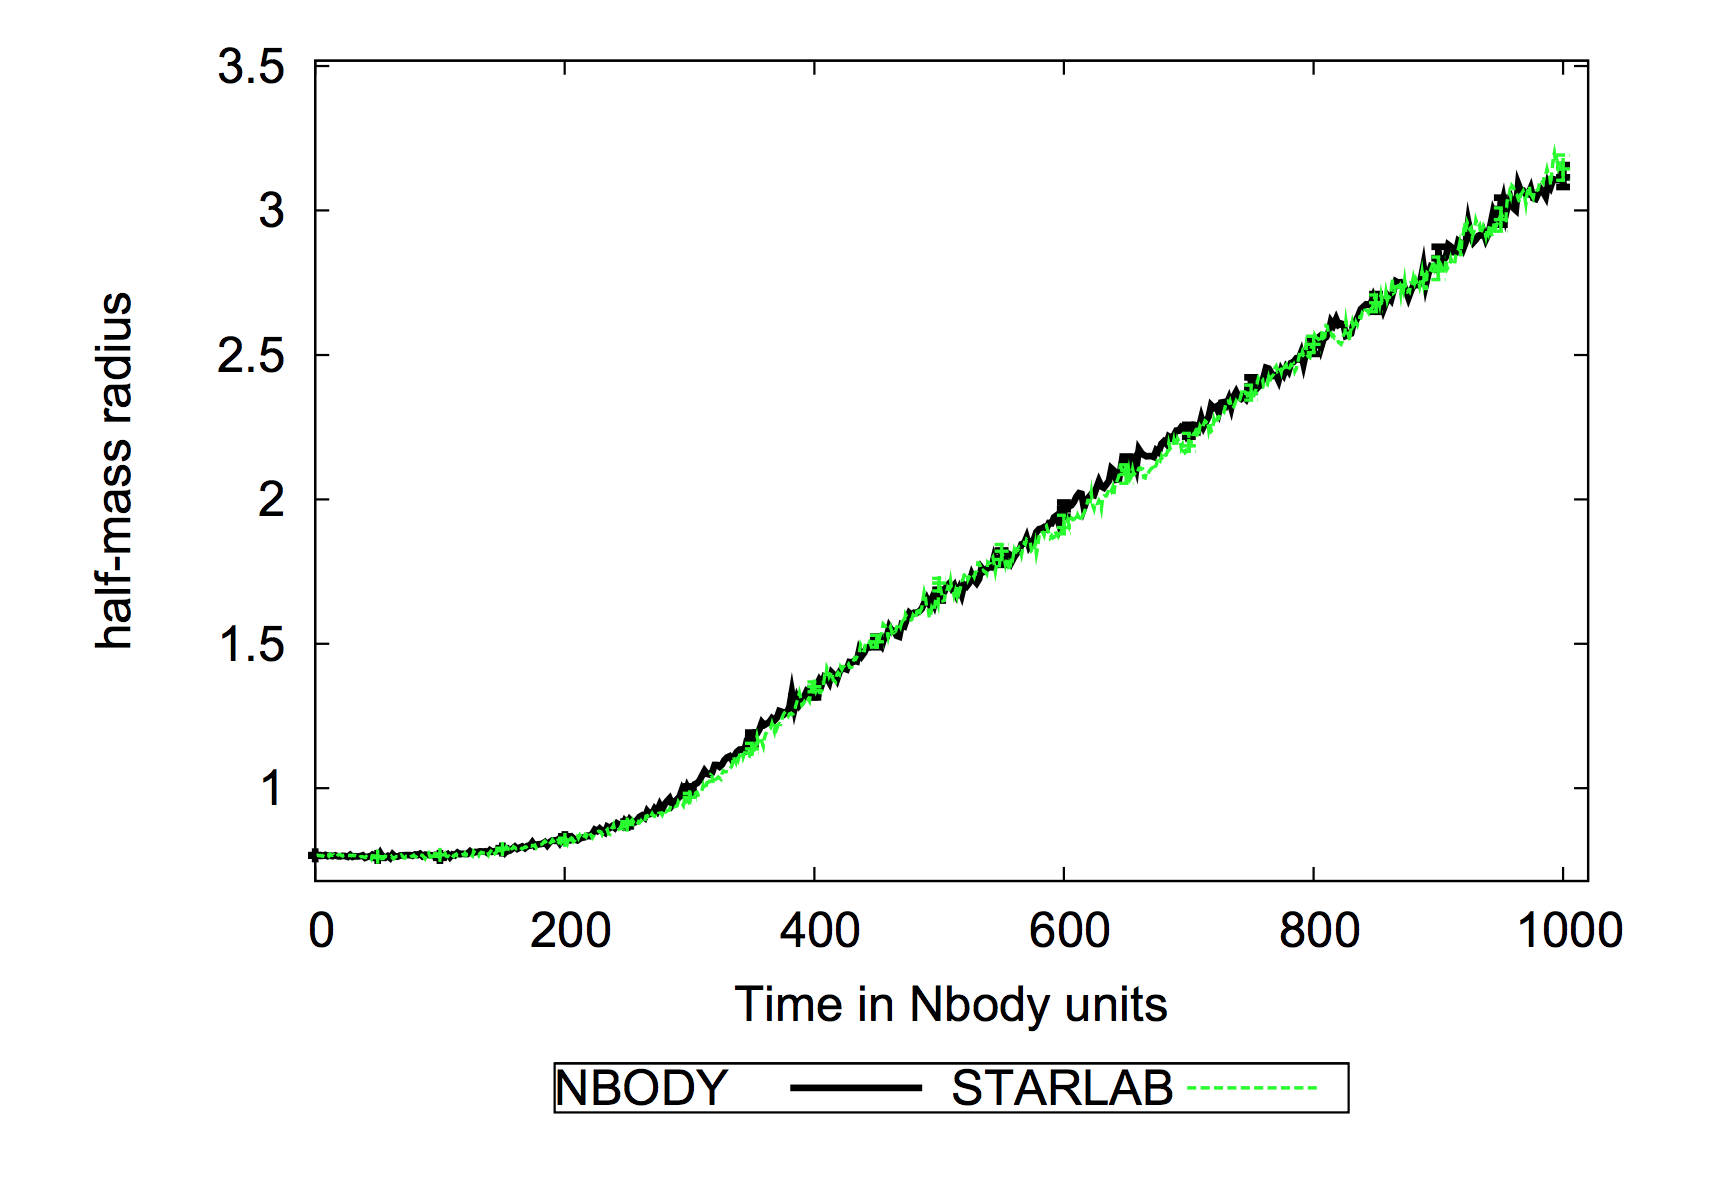
\includegraphics[width = 7cm]{AndersHalfRadius}}}%
    \qquad   
    \subfloat[Core radius vs. time reproduced from \citet{2009Anders}.]{{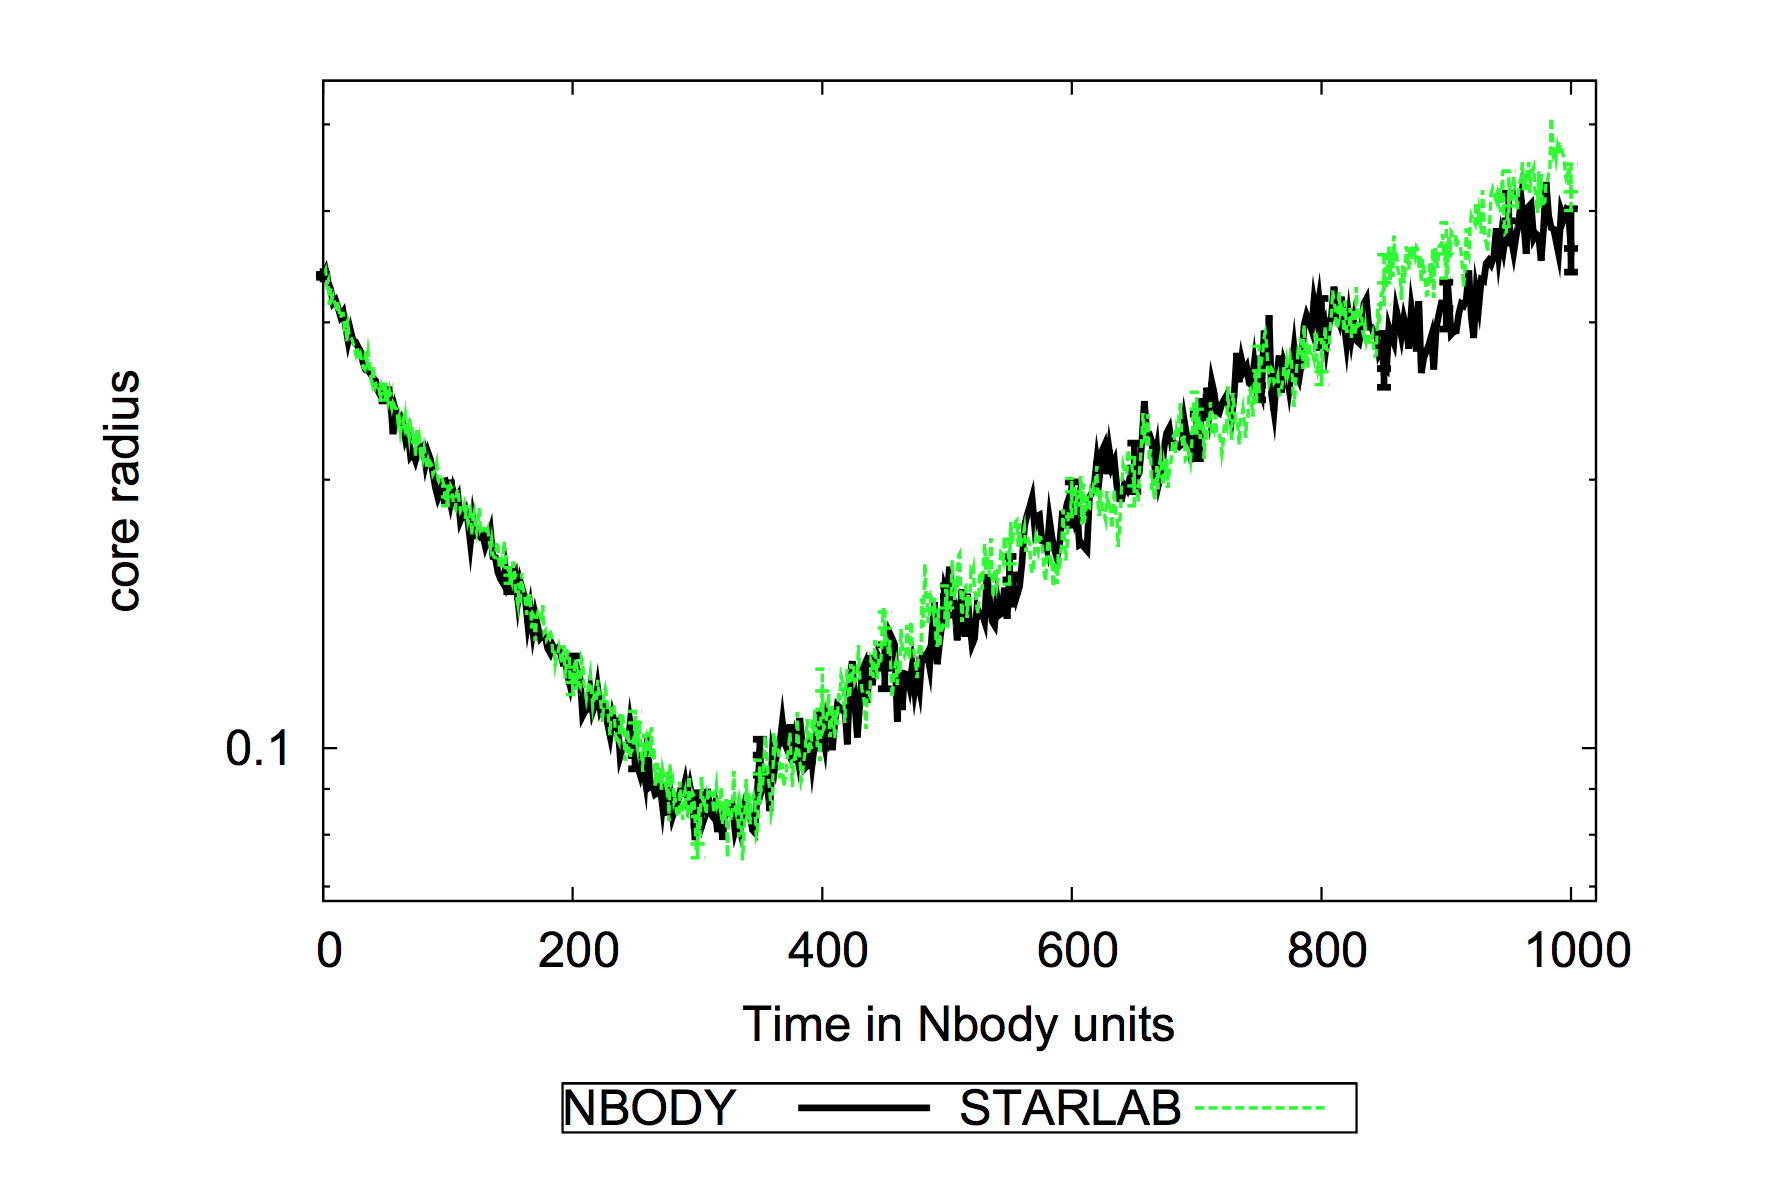
\includegraphics[width = 7cm]{AndersCoreRadius}}}%
    \qquad
    \subfloat[Half-mass radius vs. time from our verification run.]{{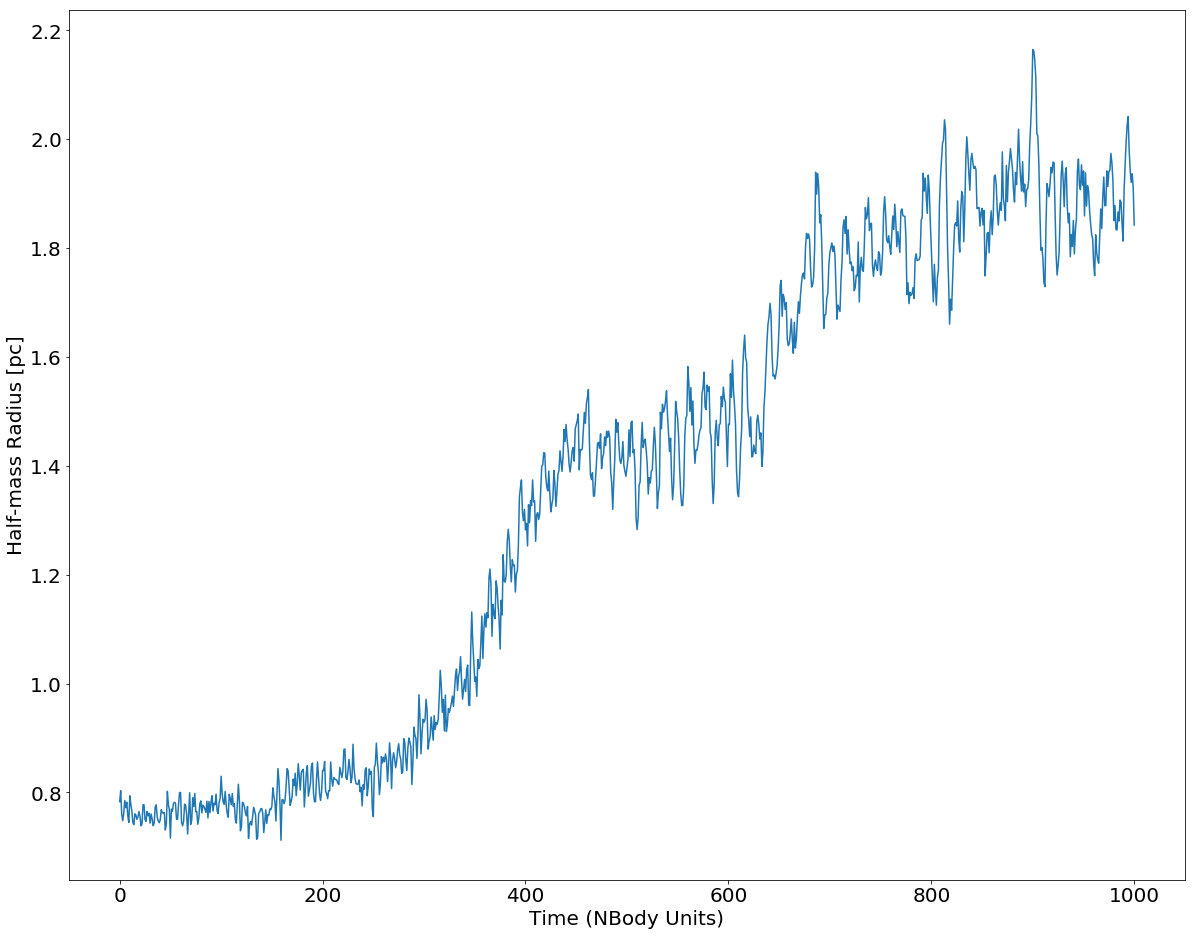
\includegraphics[width = 7cm]{VerifyHalfRadius}}}%
    \qquad
    \subfloat[Core radius vs. time from our verification run.]{{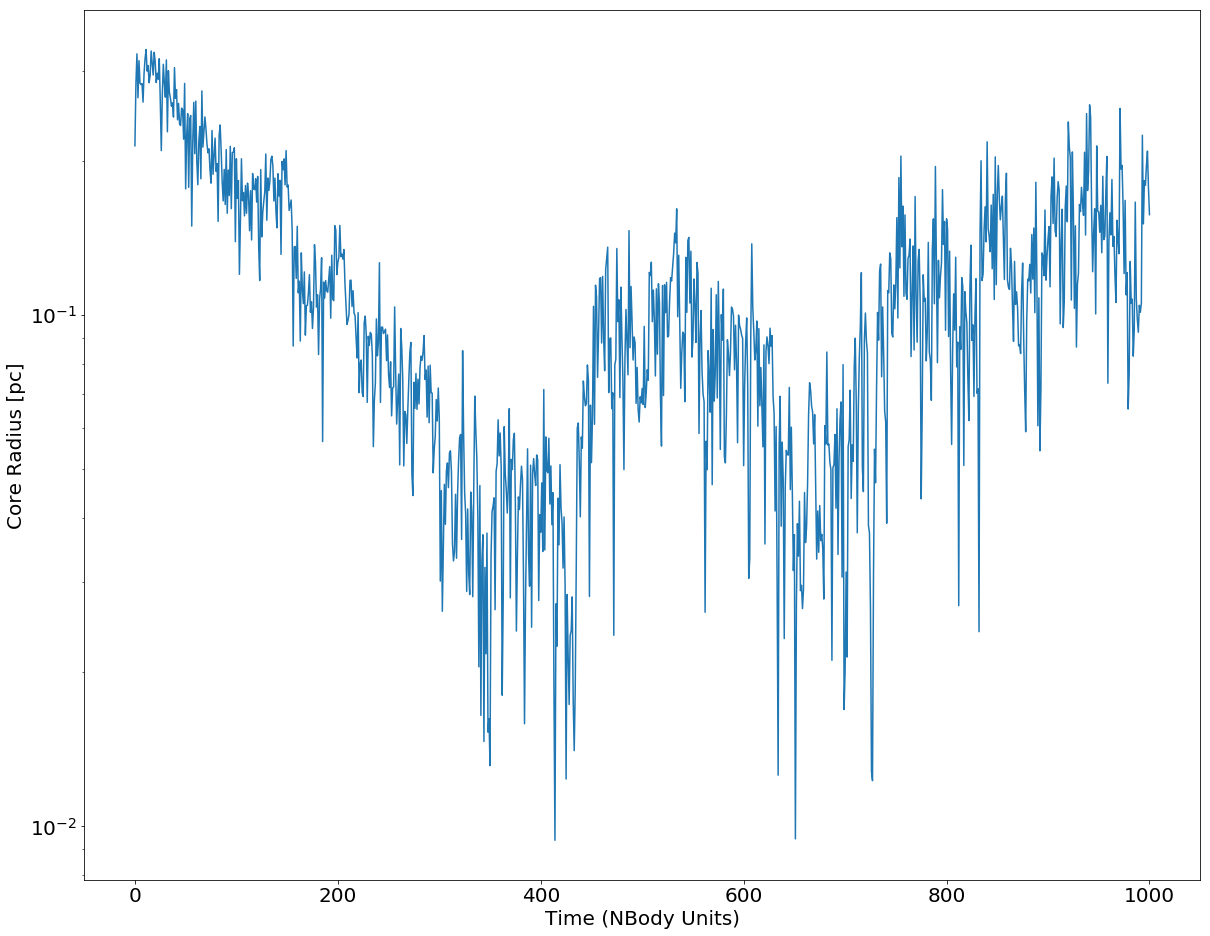
\includegraphics[width = 7cm]{VerifyCoreRadius}}}%
    \caption{Our verification run shows generally good agreement with those of \citet{2009Anders}.  The half mass radius doesn't start to expand significantly until $200$ time steps in both sets, and then follows a general upwards trend.  Our core radius shows a similar peak-trough distance of oscillation and a return close to the starting point by the end of the run.
    Our result appears to oscillate more because we show a single run instead of an entire sample. }
    \label{fig:verifications1}
\end{figure}

\begin{figure}%
    \centering
     \subfloat[Kinetic energy vs. time reproduced from \citet{2009Anders}.]{{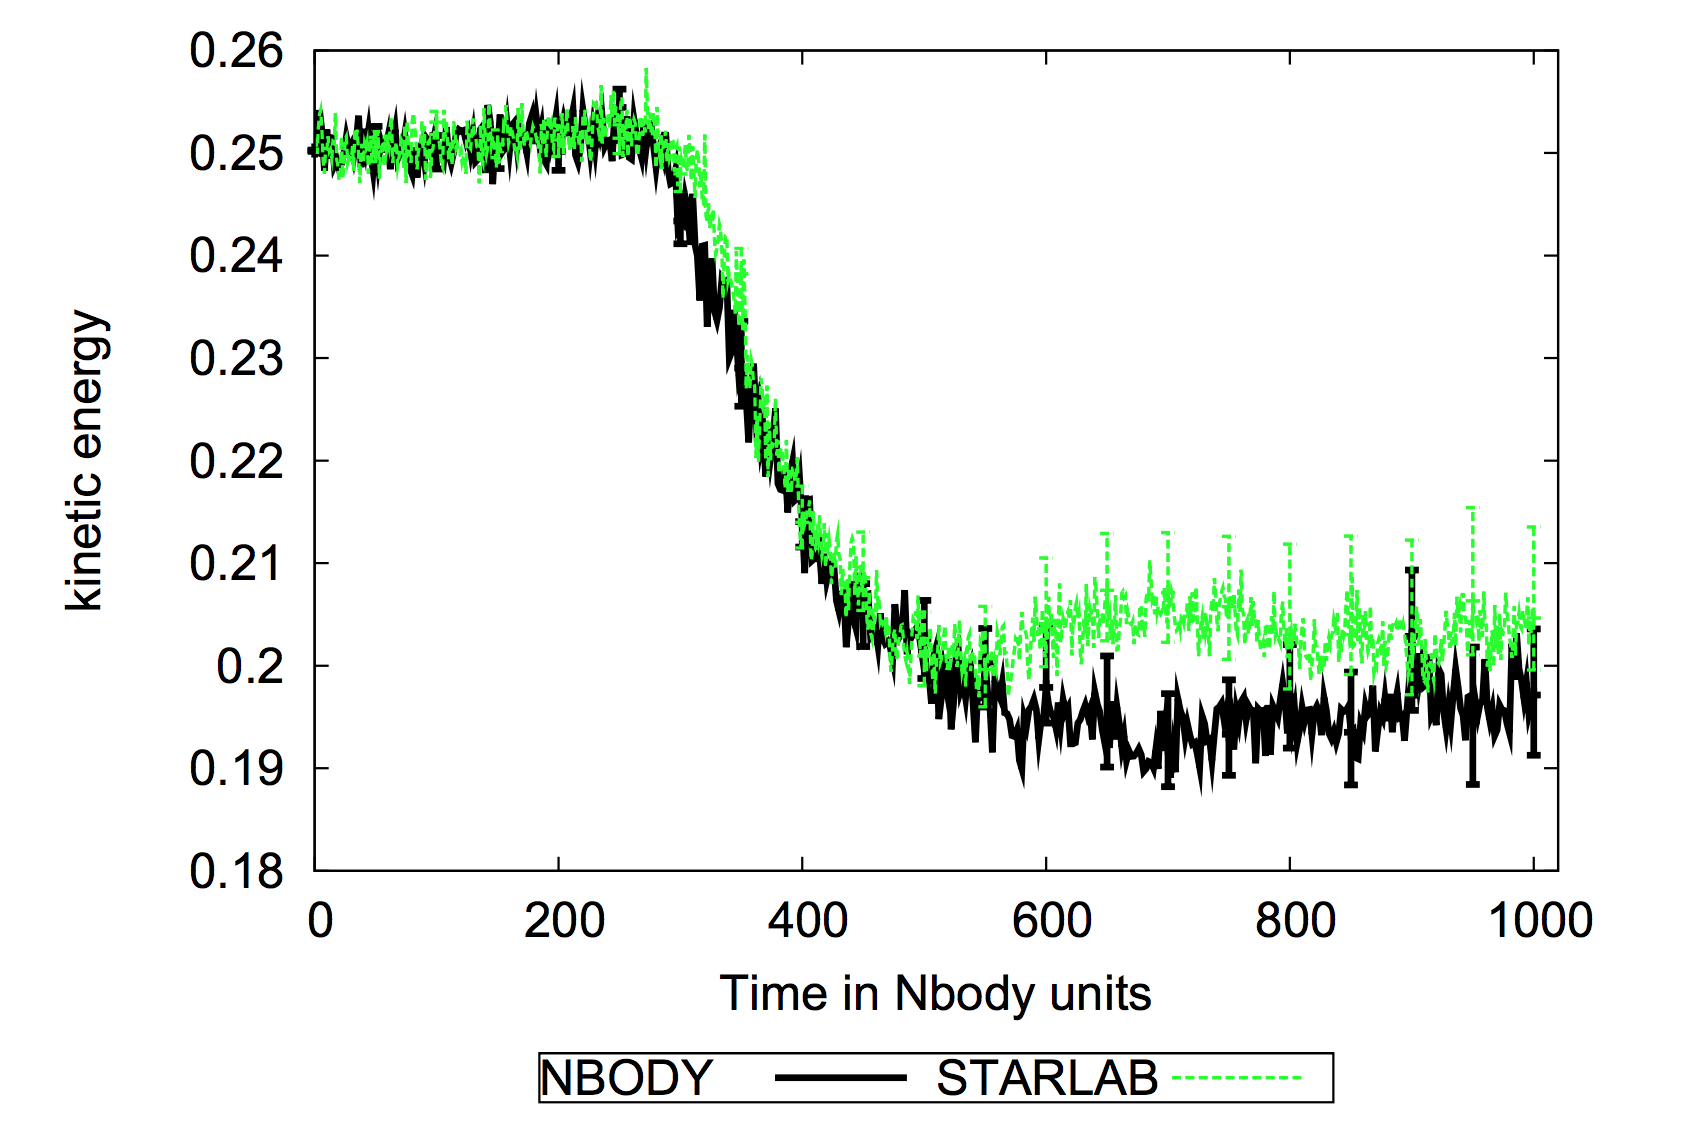
\includegraphics[width = 7cm]{AndersKinetic}}}%
    \qquad   
    \subfloat[Potential energy vs. time reproduced from \citet{2009Anders}.]{{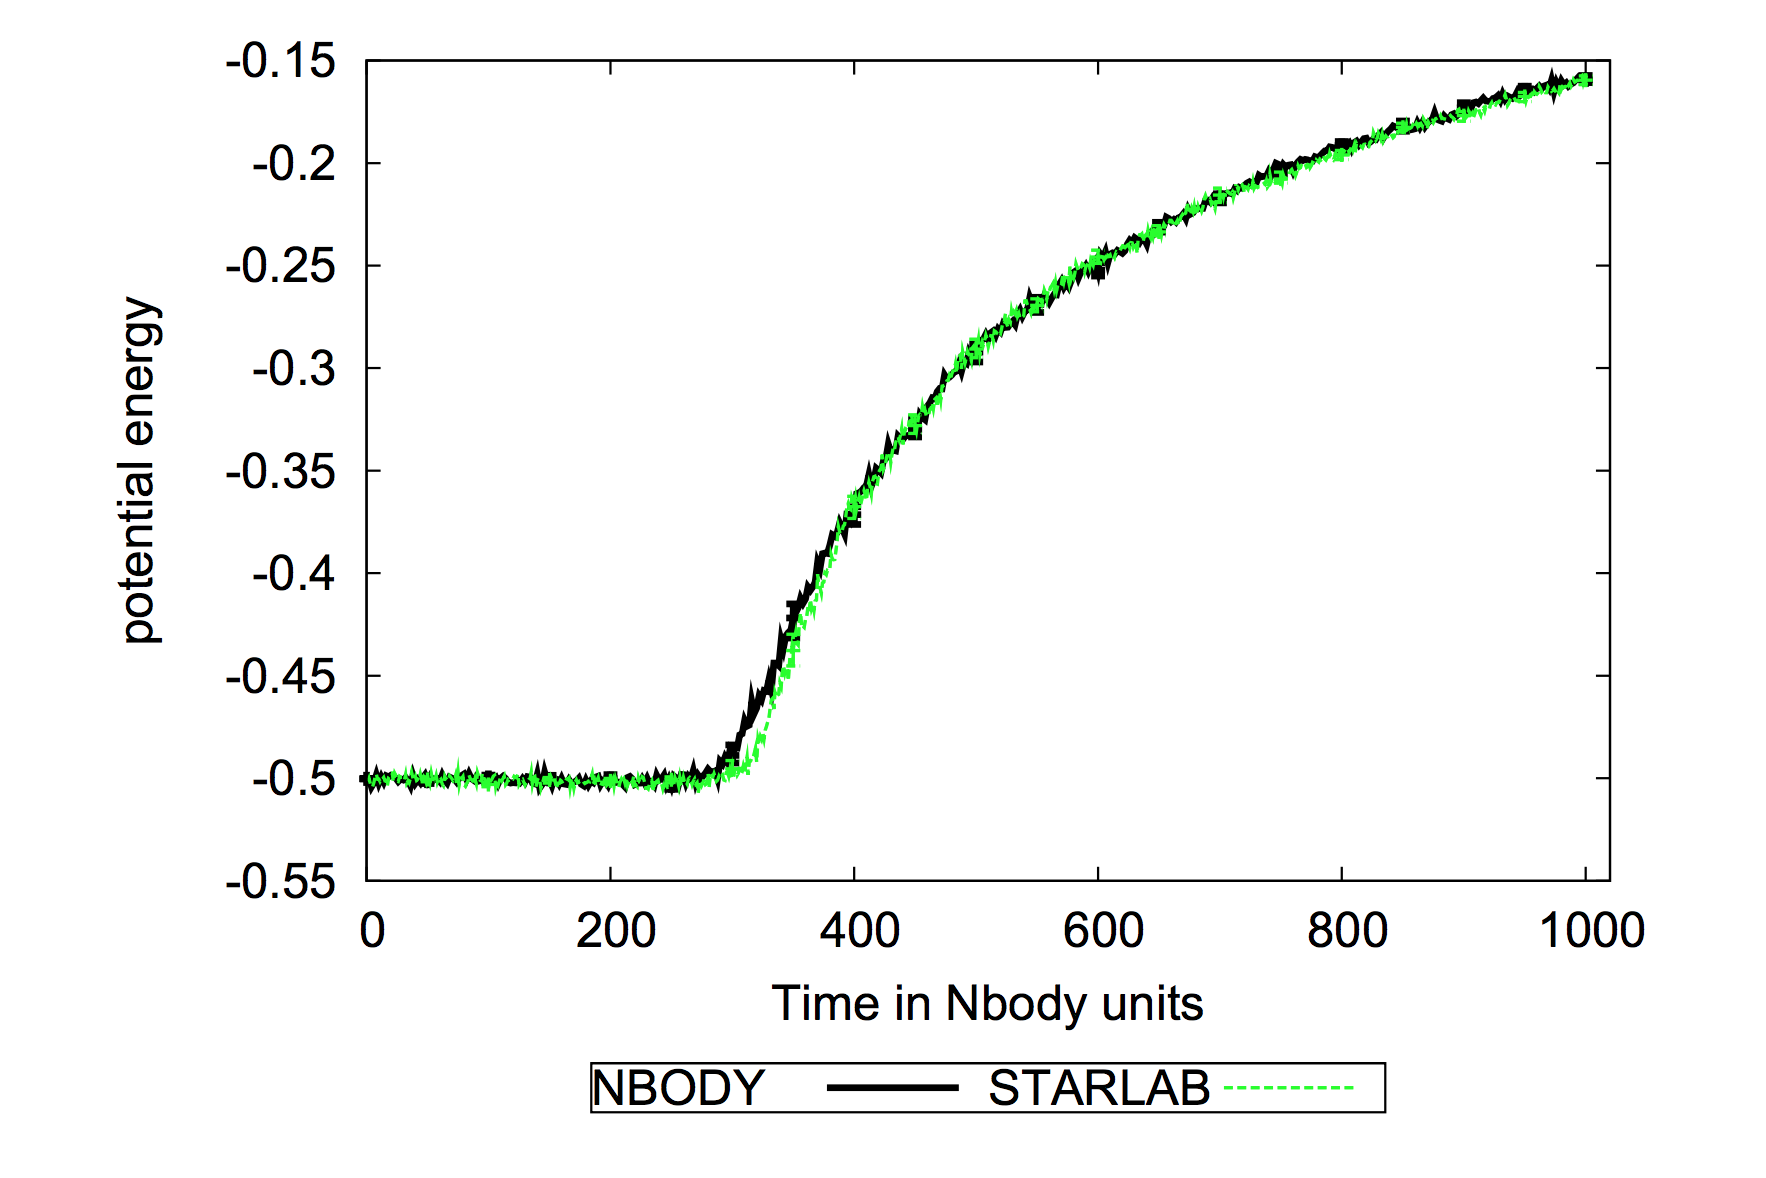
\includegraphics[width = 7cm]{AndersPotential}}}%
    \qquad
    \subfloat[Kinetic energy vs. time from our verification run.]{{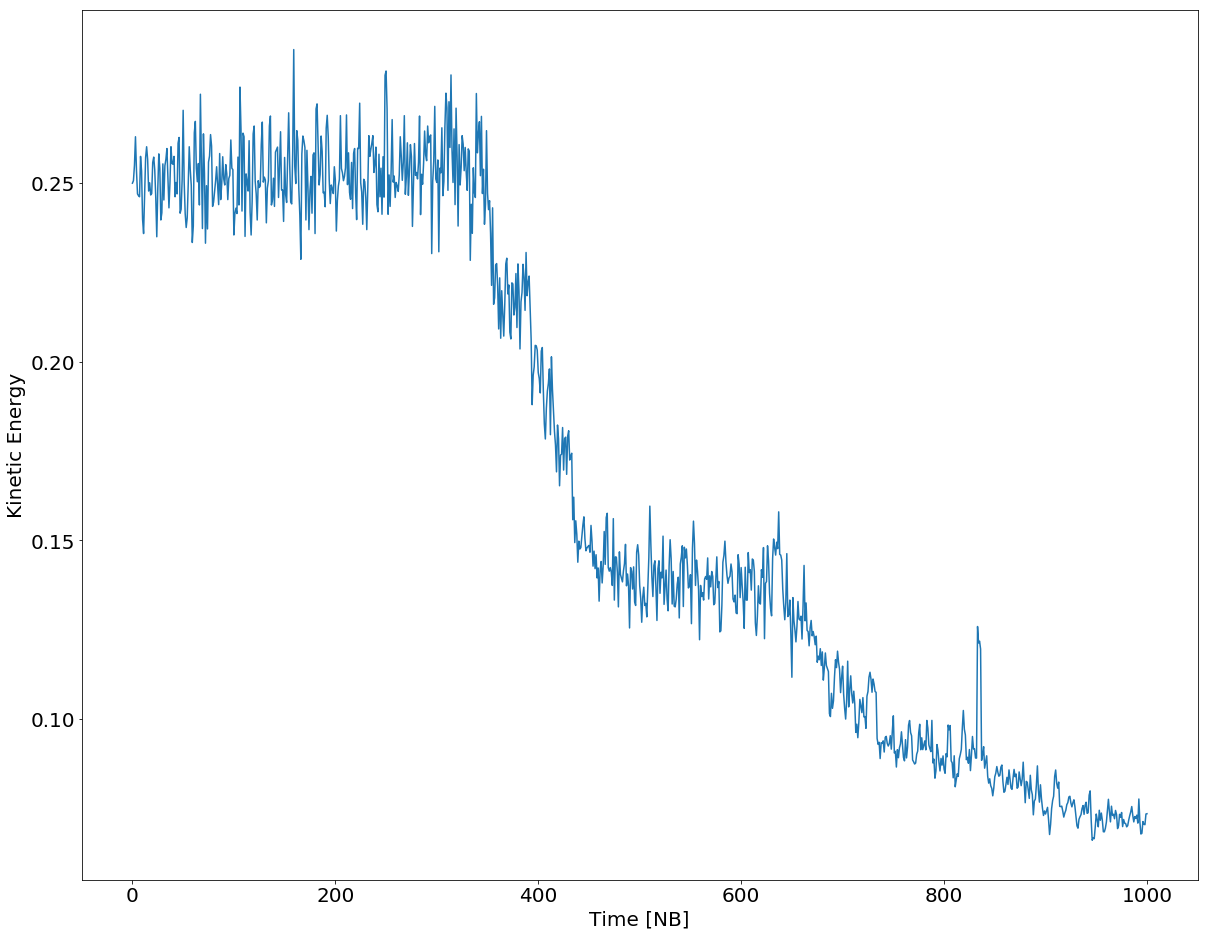
\includegraphics[width = 7cm]{VerifyKinetic}}}%
    \qquad
    \subfloat[Potential energy vs. time from our verification run.]{{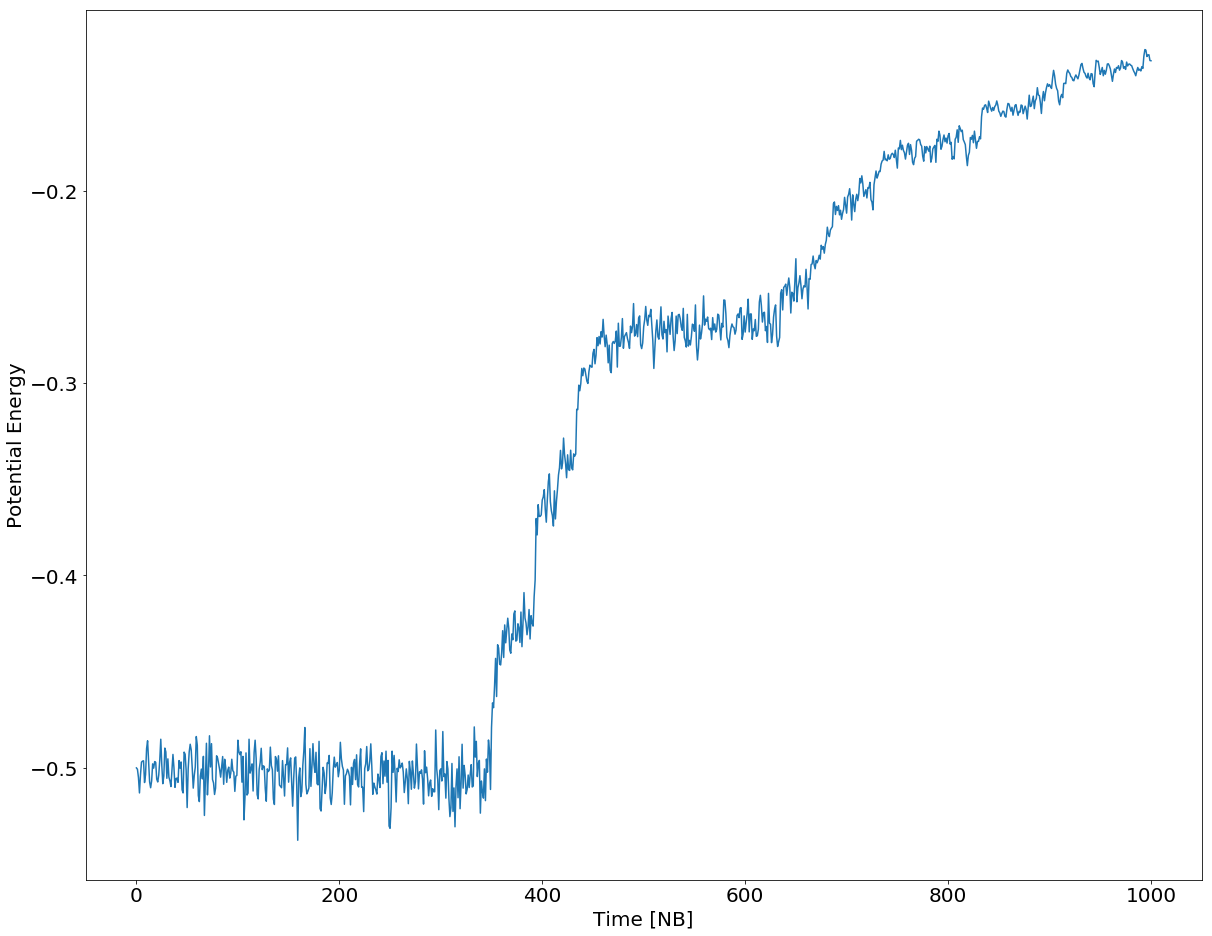
\includegraphics[width = 7cm]{VerifyPotential}}}%
    \caption{We see the same general trend with kinetic and potential energy from our verification run, although the kinetic energy from our run seems to end up lower than that of \citet{2009Anders}.  This is where there is also the greatest divergence between \texttt{NBODY4} and \texttt{Starlab}, so it's possible that changes in between \texttt{NBODY4} and \nbody account for this difference.}
    \label{fig:verifications2}
\end{figure}


\subsection{Additional Modifications}
We had significant difficulty running more collisional clusters to completion.  We found that clusters with many collisions stretched the limits of default \nbody parameters.  Among other issues, we encountered a persistent problem where runs would stop progressing during a KS regularization.  We settled on a two-part workaround for this problem: first by reducing the KS step size which seemed to forestall these failures at the cost of some additional compute time and second by simply restarting runs once they stopped progressing. 

We were unable to get \nbody's internal restart module to function in our environment, so our restart method required building a tool to parse the checkpoint data and create initial conditions for a fresh simulation.  The raw checkpoint data does not perfectly reflect the state of the system because it contains duplicate bodies when binaries, triples, quads, and chains are involved. We implemented an additional heuristic in our restart code to remove spurious binaries and other multiples, leaving only the constituent bodies in the new initial conditions.

\nbody's default configuration does not always seem to handle collisional clusters well. This led to other failure modes for our simulations which we tried to correct. In dense clusters we found that the neighbor lists would rapidly become full leading to code crashes.  Here we tried reducing the size of neighbor search spheres per the suggestion of \citet[][personal communication]{2017Wang}, which did not resolve the issue, so we instead doubled the size of the neighbor lists which was enough to alleviate the issue. Another failure mode which we have not yet been able to find a solution to occurs after restarts during GPU force initialization. It appears some initial conditions cause GPU out-of-memory errors which cause \nbody to crash. The resolution we have adopted for that failure mode is to binary search snapshots until finding one that proceeds and begin the run at that point.  We then have to invalidate data after the selected snapshot.

\section{Results} \label{Results}

\begin{sidewaysfigure}[ht]
    \centering
    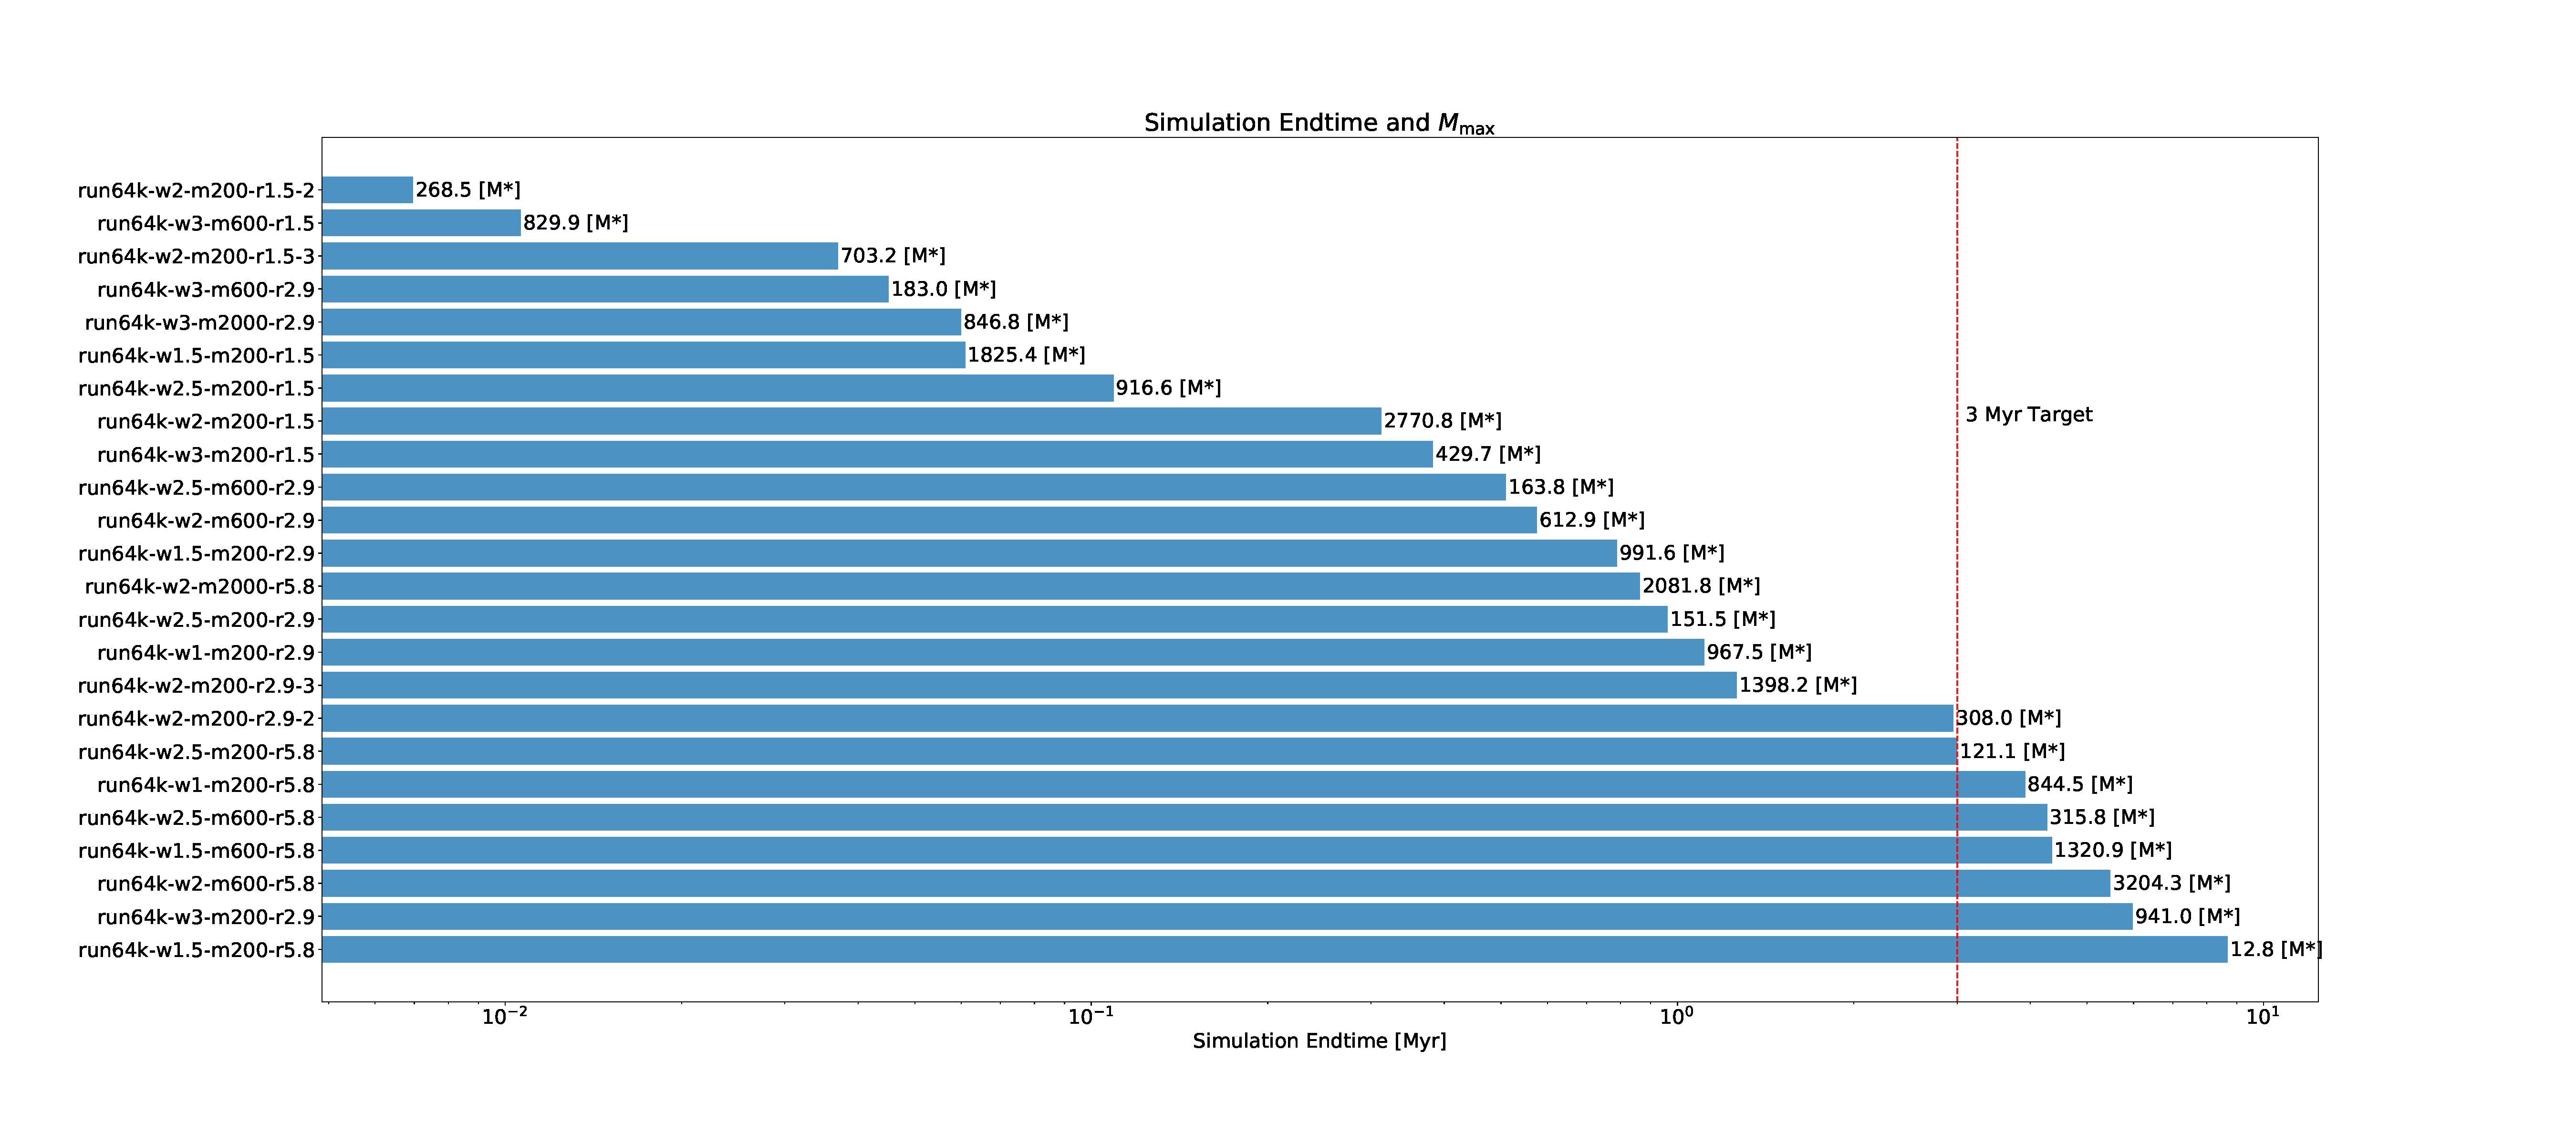
\includegraphics{JobProgress}
    \caption{Not all jobs ran to completion. }
    \label{fig:JobProgress}
\end{sidewaysfigure}

\begin{figure}
    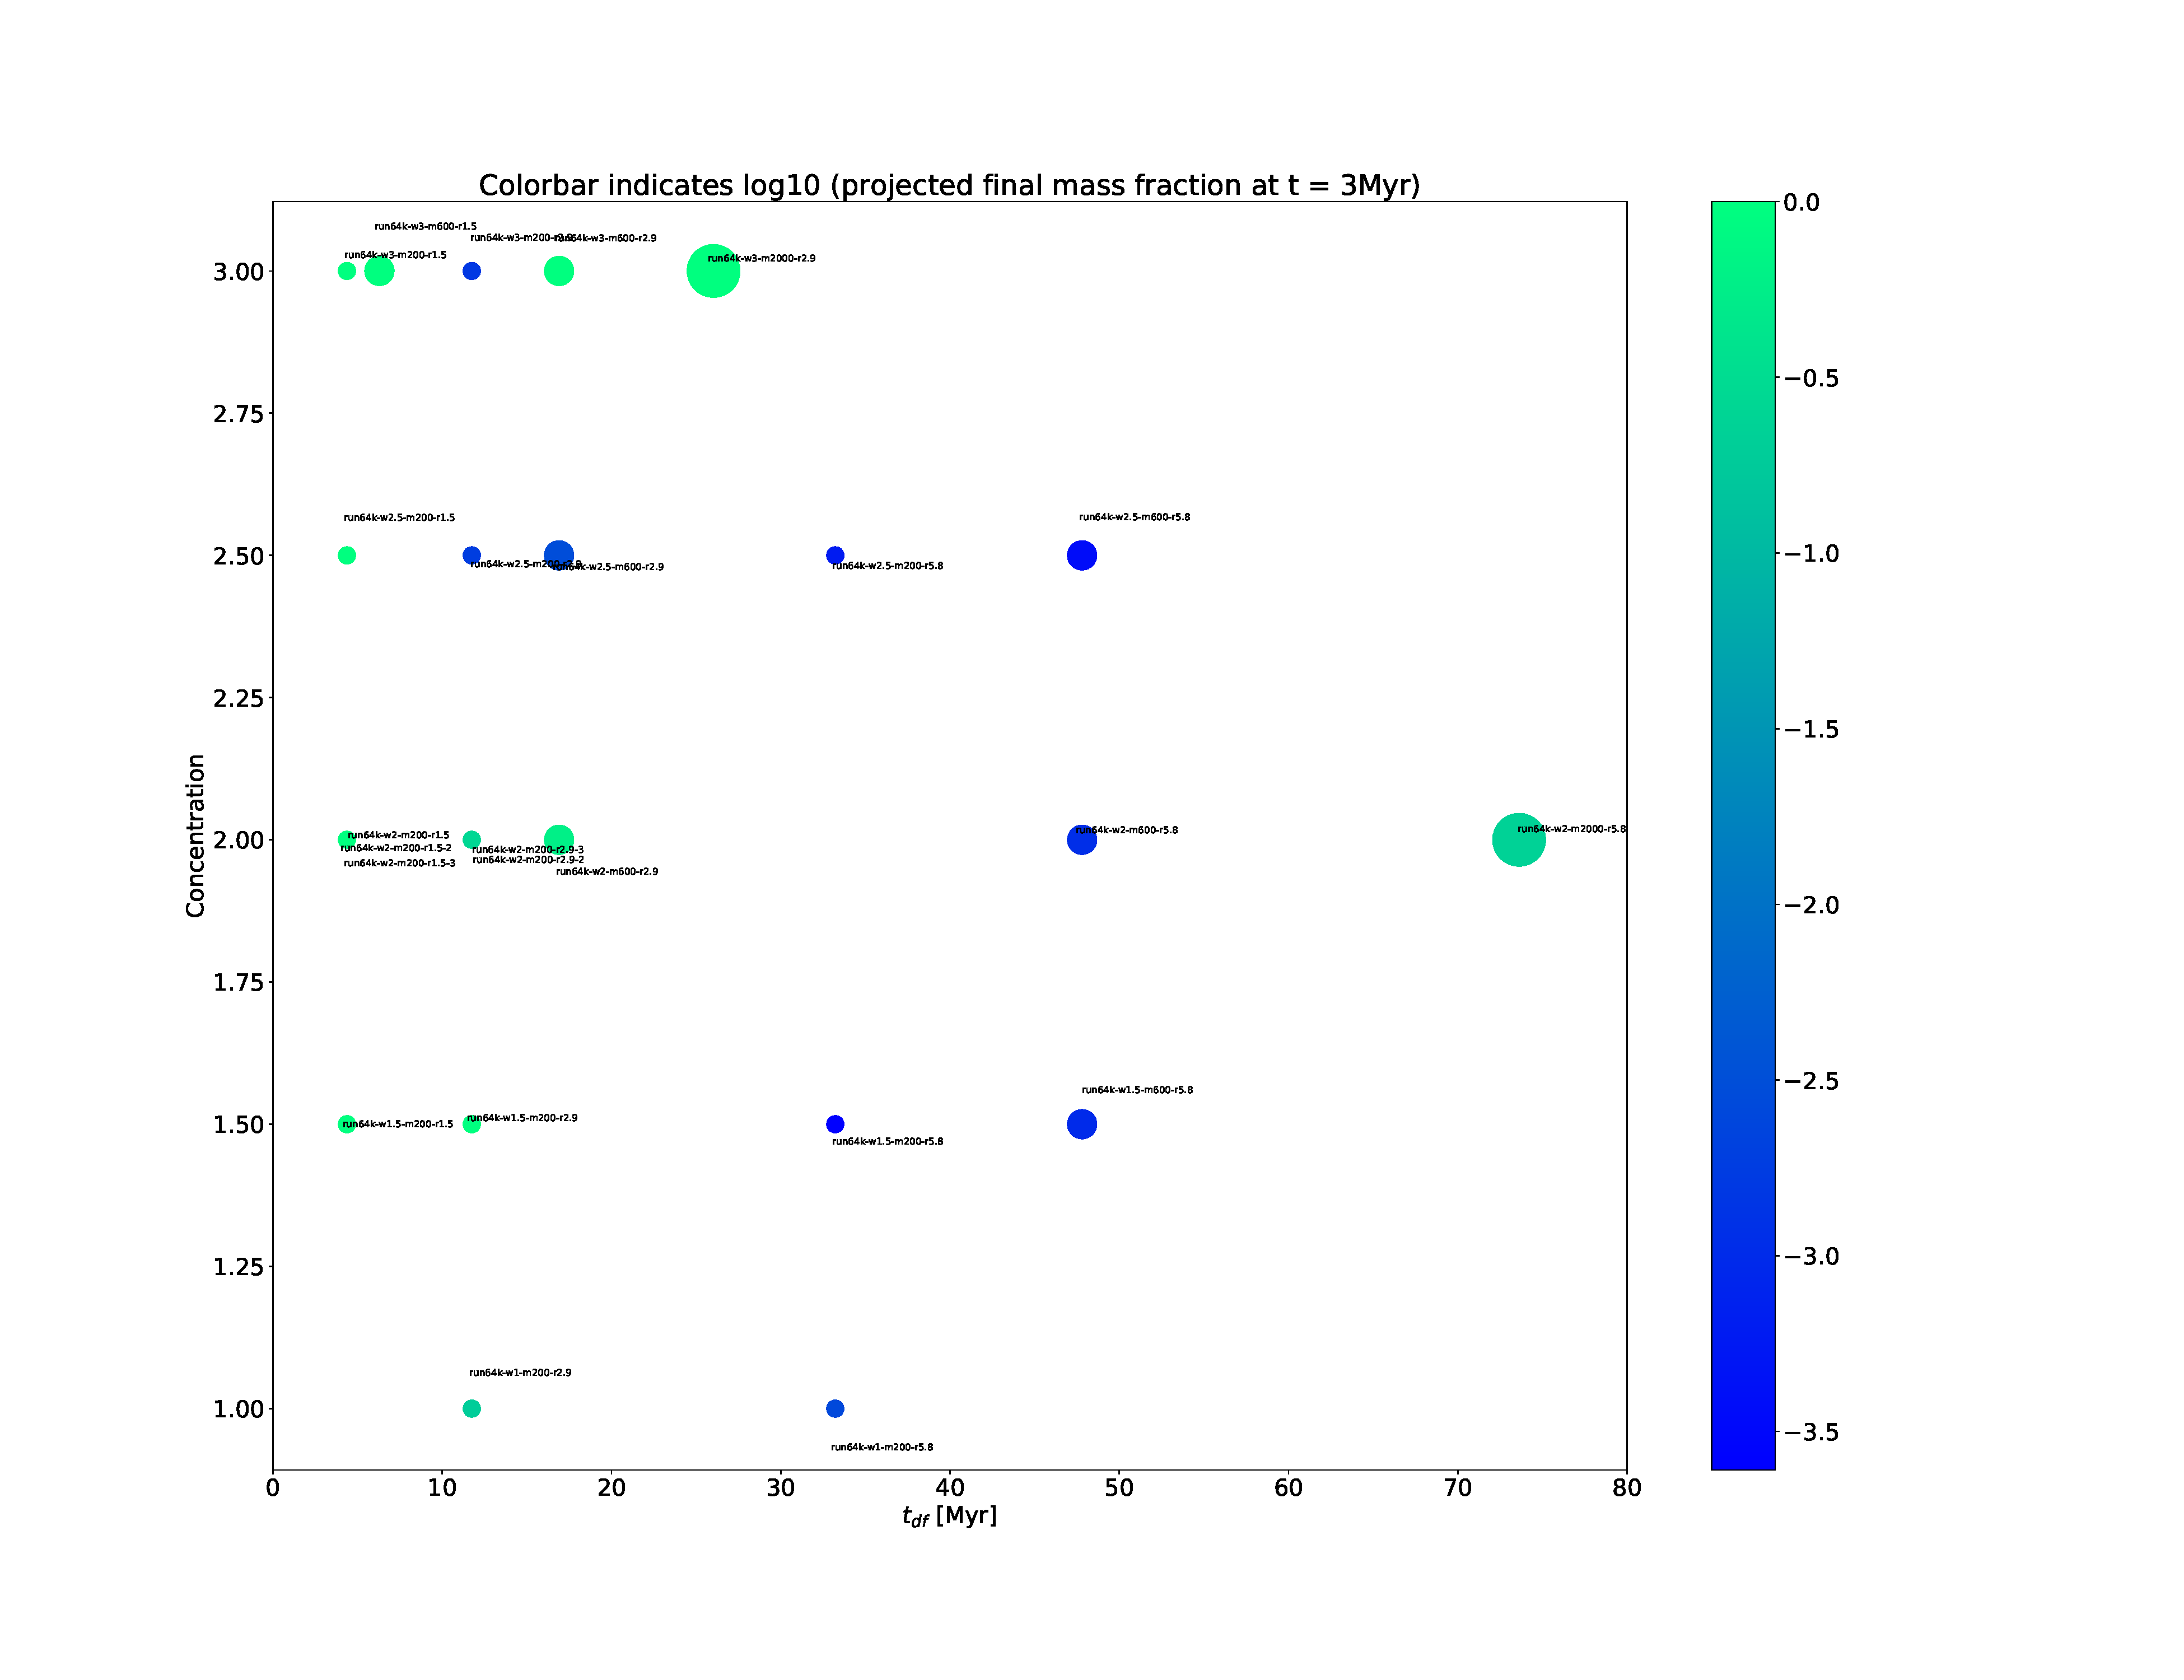
\includegraphics[width=20cm]{kplot}
    \caption{Plot of clusters with their parameter $K$}
    \label{fig:KPlot}
\end{figure}
\textbf{What clusters had runaway central masses?}
We performed simulations of 24 clusters sampling the parameter space of concentration, cluster mass, and core radius. We targeted an end time of $3 \Myr$ for each cluster to reach the end of life for the most massive stars in the cluster. Because of the computational difficulty of simulating collisional clusters with many bodies, not all of the runs made it to completion. Figure~\ref{fig:JobProgress} shows the suite of runs and their end times, as well as the size of their final central masses. As many simulations only make it to $\sim 0.1 - 0.5 \Myr$ before they become too difficult to simulate, comparing the results of different clusters requires normalizing for time.  However, we can still make a guess as to whether a runaway should occur, even if determining the exact mass of the runaway is difficult. To do this, we suppose that the early stages of cluster growth can be modeled as an exponential such that
\begin{equation}
    M_{\mathrm{max}}(t) = M_{0} e^{(Kt)}.
    \label{eqn:expcluster}
\end{equation}
We can solve for $K$ at the end of a given run by isolating it from equation~\ref{eqn:expcluster} as follows:
\begin{equation}
K = \frac{\ln M_{\mathrm{max}}(t_{\mathrm{end}}) - \ln M_{0}}{t_{\mathrm{end}}}
\end{equation}
We can then use $K$ to make an estimate for the mass fraction of the cluster at $t = 3 \Myr$.  If the projected final mass fraction is large, we suggest the cluster is a candidate to have a runaway central mass. Figure~\ref{fig:Kplot} shows each run plotted with its projected final mass fraction.  We cap this fraction at $1$.

\textbf{What fraction of the total cluster mass did the runaway achieve?  How long didit take?}

\textbf{What was the rate of growth?  Did this vary with cluster parameters?  What about the shape of the growth curves?}

\textbf{Any clusters that were too expensive to simulate or didn't work for some other reason?}

\textbf{What other observed phenomena?  Did any/all clusters experience mass loss?  What happened with core radius?  Was core collapse correlated with larger central mass?}



\bibliographystyle{apj}
\bibliography{ref}
\acrodef{SMBH}{supermassive black hole}
\acrodef{IMBH}{intermediate-mass black hole}
\end{document}
